\documentclass[12pt,a4paper]{article}

\usepackage[]{microtype}
\usepackage[utf8]{inputenc}
\usepackage[T1]{fontenc}
\usepackage[italian]{babel}
\usepackage{graphicx}
\usepackage{hyperref} %To setup table of content links
\usepackage{titlesec}
\usepackage{listings}
\usepackage{stmaryrd}

\lstset
{ %Formatting for code in appendix
    language=C,
    basicstyle=\footnotesize,
    numbers=left,
    stepnumber=1,
    showstringspaces=false,
    tabsize=1,
    breaklines=true,
    breakatwhitespace=false,
}

%\setlength{\parskip}{10pt} %Vertical space between paragraphs
\setlength{\parindent}{0pt} %Horizontal space before first line


\hypersetup{%dsadsa
    colorlinks,
    citecolor=black,
    filecolor=black,
    linkcolor=black,
    urlcolor=black
}

\newcommand{\sectionbreak}{\clearpage} %To start a section on a new page

\newcommand{\barra}{/\hspace{0pt}}

\begin{document}
\title{\textbf{Riassunto slides di Linguaggi}  \\  \large A.A. 2020-2021}
\author{Stefano Nicolis \\ stefano.nicolis@studenti.univr.it}

\maketitle

\clearpage

\tableofcontents

\clearpage

\section{Introduzione} \label{Introduzione}
\subsection{Perché studiare i linguaggi}
\begin{itemize}
\item Il linguaggio nel quale si sviluppa pone dei limiti al tipo di strutture di controllo, strutture dati e astrazioni che si possono usare, ovvero limiti agli algoritmi implementabili: conoscere più linguaggi riduce queste limitazioni
\item Invece di usare sempre lo stesso linguaggio di confidenza, programmatori più consapevoli scelgono il linguaggio con caratteristiche più adatte al problema da risolvere
\item Una comprensione degli aspetti implementativi porta ad una maggiore
comprensione del perché il linguaggio è stato progettato in un certo modo, e ci permette di usare il linguaggio in modo più intelligente ed efficiente, ovvero nel modo in cui era stato progettato per essere usato
\item Conoscere a fondo il linguaggio che usiamo, ci permette di evitare errori dovuti ad un uso inconsapevole dei suoi costrutti
\end{itemize}
\subsection{Come nascono i linguaggi}
Il principale problema dell'informatica consiste nel voler far eseguire ad una macchina algoritmi che manipolano dati.
In generale la macchina è programmabile, ovvero un calcolatore che può eseguire
insiemi di istruzioni (passi di calcolo dell'algoritmo) che chiamiamo programmi.
In particolare, i computer moderni hanno una architettura che nasce dall'architettura di \textbf{Von Neumann}. Questa è una tipologia di architettura hardware per macchine programmabili, con programma memorizzato, dove \textbf{dati ed istruzioni condividono la stessa area di memoria}.

La struttura essenziale di questa architettura \texttt{CPU + memoria} ha messo al centro del concetto di linguaggio di programmazione (oggi chiamati \textbf{linguaggi imperativi}) la \textbf{cella di memoria}. Proprio per questo lo \textbf{stato di esecuzione} di una macchina è descritto attraverso i valori contenuti nelle sue celle di memoria.

\subsection{Dal binario al linguaggio di alto livello}
A basso livello, dati e istruzioni hanno lo stesso formato: una stringa di bit può essere sia un dato che un un' istruzione. Chi legge il binario deve essere in grado di distinguere i due casi. Ciò rende molto difficile il processo di \textbf{disassemblaggio} (traduzione da binario ad assembly) e \textbf{decompilazione} (da assembly ad alto livello). Infatti, dati e istruzioni, pur essendo entrambe stringhe binarie, vanno trattati in modo sostanzialmente diverso: il dato viene \textbf{manipolato}, l'istruzione viene \textbf{interpretata}.
Per queste ragioni abbiamo bisogno di linguaggi diversi da quello binario, linguaggi che un essere umano possa facilmente capire e manipolare: questi saranno i linguaggi ad alto livello che, in modo automatico, mediante compilazione o interpretazione vengono eseguiti a livello macchina.

\subsection{Cosa significa programmare}
Un linguaggio di programmazione deve essere uno strumento che permette di \textbf{descrivere algoritmi e rappresentare dati}.

\textbf{Algoritmo}: sequenza di passi di calcolo cui significato complessivo è il calcolo di una funzione, il quale si concretizza in un programma, ovvero un insieme di frasi ben formate nel PL in questione. 

I PL Sono linguaggi formali \textbf{le cui frasi sono programmi}, ovvero forme concrete di algoritmi eseguibili/interpretabili da una macchina.

Non esiste una corrispondenza precisa tra programmi e algoritmi:
\begin{itemize}
\item Un programma non è necessariamente un algoritmo, in quanto una frase grammaticalmente corretta può non avere ``semantica utile''
\item Lo stesso algoritmo può avere concretizzazioni diverse (infinite)
\end{itemize}
\textbf{Dati}: informazioni memorizzate concretamente in celle di memoria e astratte in elementi che il linguaggio di programmazione può manipolare: le variabili.

\clearpage

\subsection{Cosa sono i linguaggi di programmazione}
Un Linguaggio di Programmazione L è un insieme di costrutti e regole per descrivere algoritmi e dati.

Il programma è la \textbf{concretizzazione} di un algoritmo che manipola dati, questa manipolazione rappresenta la \textbf{semantica} del programma (effetto del programma sui dati) mentre il programma in sè lo chiameremo \textbf{sintassi}. È necessario distinguere i due, oltre che per avere strumenti diversi per realizzarli, perché il programma è una rappresentazione finita di un insieme (potenzialmente infinito) di passi primitivi di computazione.

La componente finita è la \textbf{sintassi} mentre l'effetto potenzialmente infinito è la \textbf{semantica}.

\subsection{Progettare linguaggi}
L'architettura base dei computer ha avuto un effetto determinante nella progettazione dei linguaggi moderni di programmazione.

Il contesto in cui il linguaggio deve operare determina le funzionalità che il linguaggio deve gestire efficacemente: applicazioni scientifiche, economiche, AI, Programmazione di sistemi, Web Software.

Nuove metodologie e nuove esigenze hanno portato allo sviluppo di nuovi paradigmi e nuovi linguaggi di programmazione (come è successo per l'Object Oriented Programming).

\subsection{Aspetti di progettazione}
\begin{itemize}
\item \textbf{Leggibilità}: misura di quanto sia immediata la comprensione del programma, contribuiscono \textbf{positivamente} la semplicità del PL (pochi ed essenziali costrutti), le parole chiave significative e la progettazione ortogonale del linguaggio (ortogonale = gli elementi hanno significato indipendente dal contesto), mentre contribuisce \textbf{negativamente} la possibilità di fare la stessa cosa in più modi (overloading degli operatori)

\item \textbf{Scrivibilità}: misura di quanto è facile utilizzare il PL per creare programmi,
contribuiscono \textbf{positivamente} la possibilità di fare astrazione, l'ortogonalità ed avere modi convenienti per svolgere operazioni (librerie incluse di default), contribuiscono \textbf{negativamente} la presenza di molti costrutti, in quanto il programmatore dovrebbe conoscerli tutti per usare bene il PL

\item \textbf{Affidabilità e costo}: misura di quanto un programma sia conforme alle sue specifiche (è affidabile se, data una qualsiasi condizione, fa sempre quello che deve), e di quanto costi (tempo e soldi) la creazione e mantenimento del programma (formazione dei programmatori, compilazione, esecuzione e mantenimento del codice)
\end{itemize}

\subsection{Classificazione dei linguaggi}
Inizialmente (anni 50-60) lo sviluppo di PLs era incentrato sulle caratteristiche di base (strutture di controllo, efficienza esecuzione, \ldots), mentre nei decenni successivi, stabilite le basi, ci si concentrò sullo sviluppo di linguaggi specifici per diversi ambiti\slash problemi (OOP, Concorrenti, Distribuiti, Scripting, Interpretati, \ldots).

Vediamo come si classificano i linguaggi in base al livello di astrazione dei propri costrutti rispetto all'HW su cui girano.
\begin{itemize}
\item \textbf{Basso livello}: caratteristiche dipendenti dall'architettura, ho pochi\slash nessun costrutto, scrivo tutto da zero (binario, Assembly)
\item \textbf{Alto livello}: i dati ed istruzioni hanno rappresentazioni diverse
\begin{itemize}
\item \textbf{Imperativi}: si basano su Von Neumann, ovvero la cella di memoria, dove la variabile è l'astrazione logica della cella, mentre l'assegnamento è l'operazione primitiva di modifica della cella e quindi dello stato della macchina
\item \textbf{Funzionali}: più vicini alla matematica descrivono i passi di calcolo come funzioni e composizioni di esse, una variabile è un nome per qualcosa e non cambia
\item \textbf{Logici}: regole e assiomi rendono possibile specificare il processo di computazione, fanno pattern-matching, come passo di calcolo primitivo usano l'unificazione\slash sostituzione, permettono di rappresentare formalmente oggetti infiniti in modo finito, ma non computazioni infinite
\item \textbf{Matematici}: Notazione rigorosa per rappresentare funzioni ma non sempre oggetti e computazioni infinite
\end{itemize}
\end{itemize}

\clearpage

\subsection{Implementare linguaggi}
Implementare un linguaggio significa renderlo comprensibile alla macchina che deve eseguirne i programmi.
Il funzionamento di tale macchina consiste in un ciclo che costituisce l'\textbf{interprete} del linguaggio che la macchina riconosce, ovvero:
\begin{itemize}
\item \textbf{Fetch}: viene letta l'istruzione dalla memoria
\item \textbf{Decode}: viene decodificata l'operazione e, se richiesti, recuparti gli operandi necessari
\item \textbf{Execute}: viene eseguita l'istruzione e memorizzato il risultato
\end{itemize}
Quando usiamo un linguaggio di programmazione \textbf{ad alto livello} lavoriamo su una macchina, chiamata \textbf{macchina astratta}, che interpreta le istruzione del PL in questione. Questo ci permette, da un certo livello di astrazione in poi, di ignorare completamente l'esistenza della macchina fisica e del suo linguaggio binario.
Quindi possiamo dire che \textbf{implementare un linguaggio significa realizzare la macchina astratta che interpreta il linguaggio}. Tale macchina è la combinazione di una memoria che immagazzina i programmi e di un interprete che esegue le istruzioni dei programmi.

Il linguaggio \texttt{L}, riconosciuto (interpretato) dalla macchina astratta \texttt{ML} viene anche chiamato \textbf{linguaggio macchina}: formalmente è l'insieme di tutte le stringhe interpretabili da \texttt{M}.

\subsection{Dove realizzare la macchina astratta}
Una qualsiasi macchina astratta per \texttt{L}, per essere eseguita, deve prima o poi utilizzare qualche dispositivo fisico che concretamente esegue le istruzioni di \texttt{L}.
Le macchine astratte possono essere realizzate a diversi livelli:
\begin{itemize}
\item \textbf{HW}: sempre possibile e concettualmente semplice. Si realizza mediante dispositivi fisici, il linguaggio macchina è il linguaggio fisico\slash binario.
\item \textbf{FW}: consiste nella simulazione delle strutture dati e degli algoritmi in \texttt{M} mediante microprogrammi. Il linguaggio macchina microprogrammato è a basso livello e consiste di microistruzioni che specificano semplici operazioni di trasferimento dati tra registri, da\slash per la memoria principale ed eventualmente attraverso circuiti logici che realizzano operazioni aritmetiche. I microprogrammi risiedono in speciali aree di memoria di sola lettura. Veloce e più flessibile della realizzazione HW.
\item \textbf{SW}: realizzazione delle strutture dati e degli algoritmi di \texttt{M} mediante programmi scritti in un altro linguaggio \texttt{L'} che possiamo supporre già implementato. Ovvero, avendo la macchina astratta per \texttt{L'}, possiamo realizzare quella per \texttt{L} mediante opportuni programmi scritti in \texttt{L'} che interpretano i costrutti di \texttt{L} simulando le funzionalità di \texttt{M} per \texttt{L}. Riduce la velocità ma aumenta la flessibilità.
\end{itemize}

\subsection{Livelli di astrazione}
Ogni sistema SW moderno ha una struttura suddivisa a livelli di astrazione cooperanti, sequenziali e indipendenti. Ciascun livello è definito da un linguaggio \texttt{L} che è l'insieme delle istruzioni che il livello mette a disposizione per i livelli successivi\slash superiori. Tutte le istruzioni di un linguaggio ad un livello \texttt{i} sono implementate da programmi a livello \texttt{j<i}.

\begin{figure}[h!]
	\begin{center}
	  \fbox{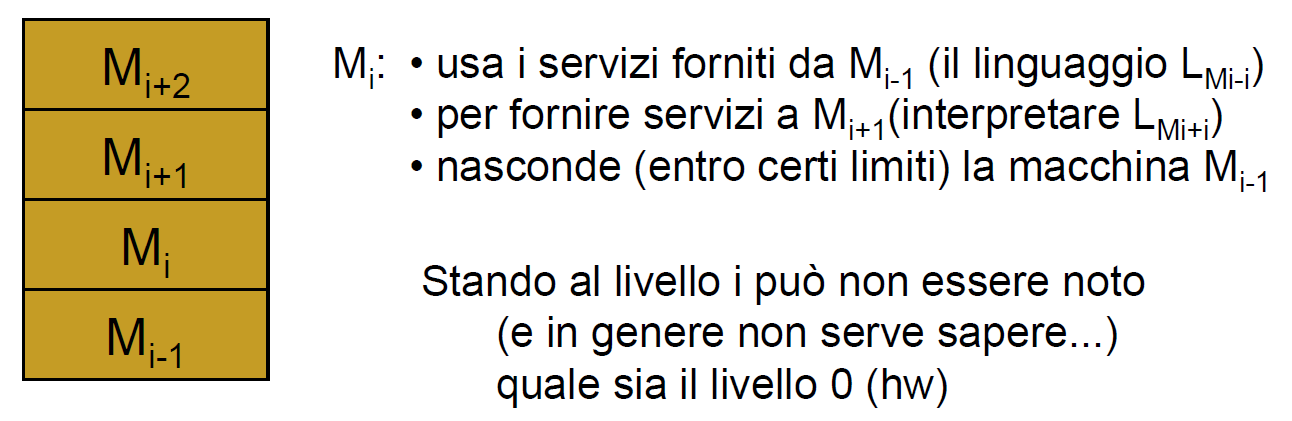
\includegraphics[scale=0.3]{media/livelli_astrazione_macchine}}
	\end{center}
\end{figure}

\clearpage

\subsection{Come realizzare la macchina astratta}
La corrispondenza tra Linguaggio \texttt{L} e Macchina che lo sa eseguire \texttt{ML} non è biunivoca: una macchina astratta corrisponde univocamente ad un linguaggio, il suo linguaggio macchina, ma dato un linguaggio \texttt{L} esistono infinite macchine astratte che hanno
come linguaggio macchina esattamente \texttt{L}. Tali macchine differiscono nel modo in cui la macchina astratta viene realizzata e nelle strutture dati utilizzate.

Realizzare \texttt{ML} consiste in realizzare \textit{una} macchina che ``traduce'' \texttt{L} in \texttt{L0} (\texttt{L0} linguaggio macchina), ovvero che interpreta tutte le istruzioni di \texttt{L} come (sequenza di) istruzioni di \texttt{L0}. Possiamo distinguere due modalità radicalmente diverse a seconda del fatto che si abbia una traduzione ``\textbf{implicita}'' realizzata dalla \textbf{simulazione dei costrutti} di \texttt{ML} (ovvero di \texttt{L}) mediante programmi scritti in \texttt{L0}, soluzione chiamata \textbf{interpretazione}, oppure si abbia un una traduzione ``\textbf{esplicita}'' dei programmi di \texttt{L} in corrispondenti programmi di \texttt{L0}, soluzione chiamata \textbf{compilativa}.

\subsubsection{Interpretazione}
L'interprete esegue ogni istruzione di \texttt{L} simulandola usando un certo insieme di istruzioni di \texttt{L0}. Questa non è una vera traduzione in quanto il codice in \texttt{L0} viene eseguito istruzione per istruzione, e non tradotto per intero e poi eseguito.

Alcuni linguaggi interpretati sono JavaScript, PHP, Python.

Le operazioni che l'interprete esegue per simulare le istruzioni del linguaggio sono:
\begin{itemize}
\item \textbf{Elaborazione dei dati primitivi}: gestione delle operazioni sui dati primitivi (\texttt{int, float, bool,}\ldots)
\item \textbf{Controllo di sequenza delle esecuzioni}: gestione del flusso di esecuzione delle istruzioni, ovvero calcolare la prossima istruzione da eseguire, non sempre sequenziale
\item \textbf{Controllo dei dati}: operazioni che permettono il recupero dalla memoria e la gestione degli operandi necessari per eseguire le istruzioni
\item \textbf{Controllo della memoria}: gestione delle operazioni di accesso e allocazione\slash deallocazione della memoria
\end{itemize}

\begin{figure}[h!]
	\begin{center}
	  \fbox{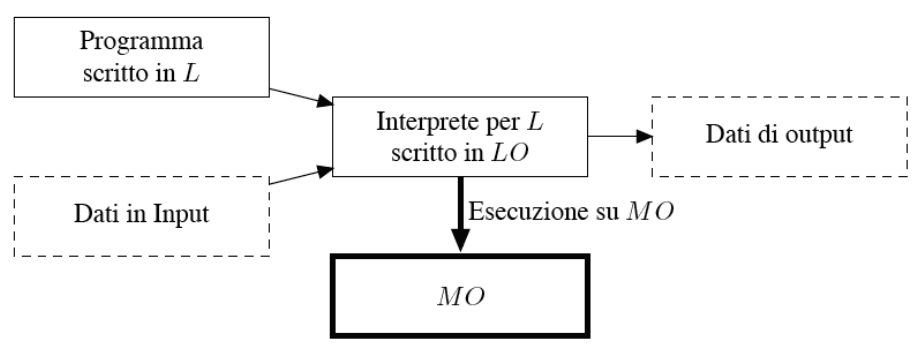
\includegraphics[scale=0.4]{media/interpretazione}}
	  \caption{Struttura interprete}
	\end{center}
\end{figure}

\begin{figure}[h!]
	\begin{center}
	  \fbox{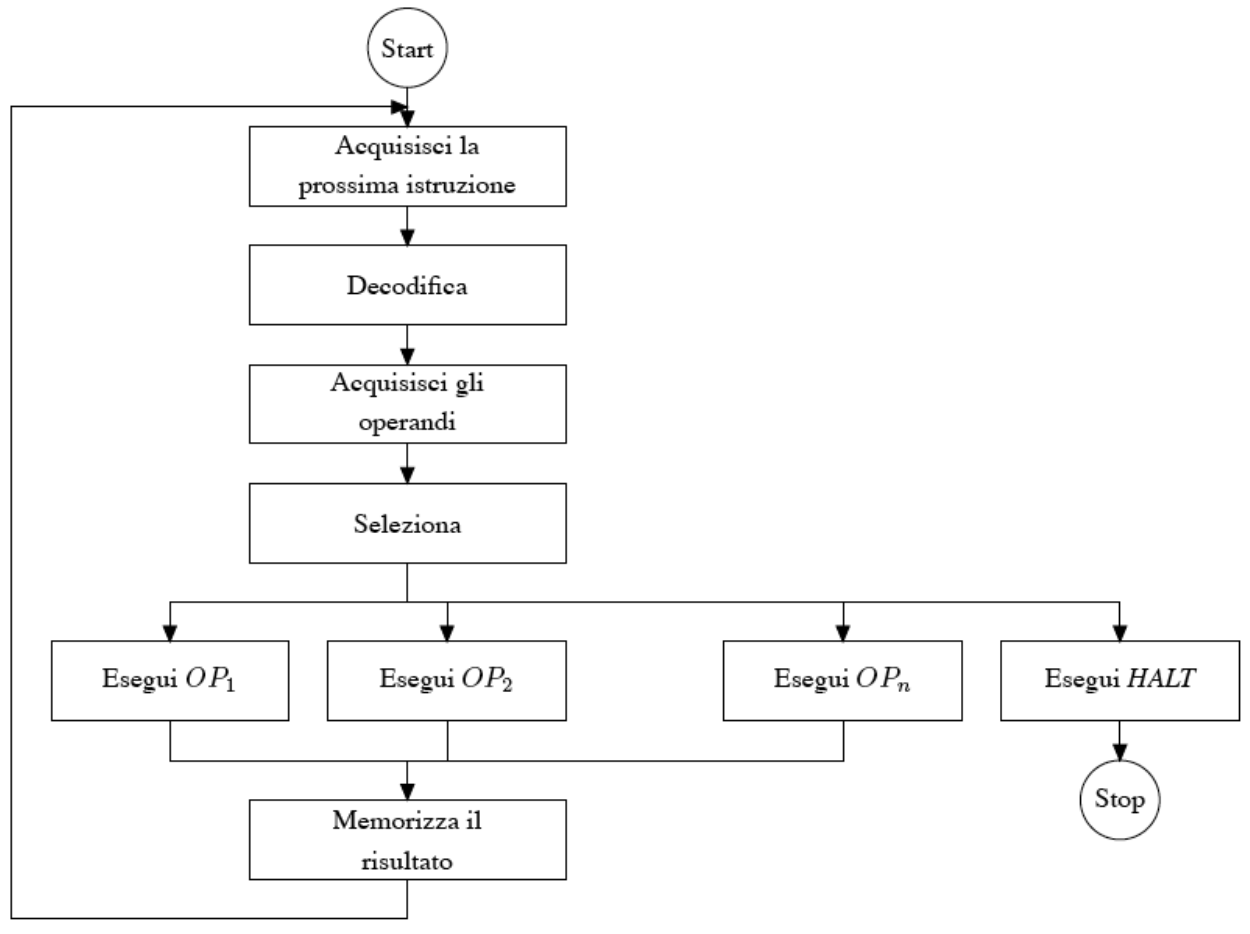
\includegraphics[scale=0.4]{media/struttura_interpete}}
	  \caption{Flusso di esecuzione interprete}
	\end{center}
\end{figure}

\clearpage

\textbf{Definizione}: Dato un programma $P$ scritto nel linguaggio $L$, $P^L \in Prog^L$ e dati in input $in \in D$, un interprete per $L$ scritto in $L0$, $int^{L,L0}$ è un programma tale che $\llbracket int ^{L,L0} \rrbracket : (Prog^L \times D) \longrightarrow$ D e

\begin{center}
\texttt{$ \llbracket int ^{L,L0} \rrbracket (P^L,in) = \llbracket P^L \rrbracket (in)$ }
\end{center}

Dove:
\begin{itemize}
\item $Prog^L$ è l'insieme dei programmi scritti in L
\item D è l'insieme di dati (input e output)
\end{itemize}

A parole, un interprete è un programma $int ^{L,L0}$ che esegue, sulla
macchina astratta per $L0$, programmi $P^L$ scritti in $L$ su un fissato input $in\in D$. Quindi è una macchina universale che preso un programma e un suo input, lo esegue su quell’input, usando solo funzionalità messe a disposizione dal livello (macchina astratta) sottostante.
\subsubsection{Compilazione}
Un compilatore è un programma che prende in input un programma in \texttt{L} e lo traduce \textbf{per intero} (preservandone la semantica) in un programma scritto in \texttt{L0}, e quindi eseguibile direttamente sulla macchina astratta per \texttt{L0}. Il processo di compilazione avviene sulla macchina astratta.

Alcuni linguaggi compilati sono \texttt{C}, \texttt{C++}, \texttt{Pascal}.

Le operazioni che il compilatore esegue per la traduzione del programma sono:
\begin{itemize}
\item \textbf{Analisi lessicale (Scanner)}: spezza un programma nei componenti sintattici primitivi chiamati \textbf{tokens} (identificatori, numeri, parole riservate, \ldots), i quali formano linguaggi regolari.
\item \textbf{Analisi sintattica (Parser)}: crea una \textbf{rappresentazione ad albero} della sintassi del programma dove ogni foglia è un token e le foglie lette da sx a dx costituiscono le frasi scritte originariamente (ben formate si spera) del linguaggio. Quando non è possibile costruire l'albero significa che qualche frase è \textbf{illegale}. In tal caso la compilazione si blocca con un errore. Le frasi di token formano \textbf{linguaggi Context-Free}.
\item \textbf{Analisi Semantica (Generazione codice intermedio e ottimizzazione)}: si verificano aspetti vicini alla semantica ma che si verificano sulla sintassi, come il Type checking e  l'equivalenza del numero di parametri tra la definizione e la chiamata di una funzione. Se previsto, si ottimizza il codice intermedio mediante l'eliminazione di codice morto, valutazione a priori delle espressioni, \ldots
\item \textbf{Generazione codice oggetto}: generazione del codice finale risultato della compilazione
\end{itemize}

\begin{figure}[h!]
	\begin{center}
	  \fbox{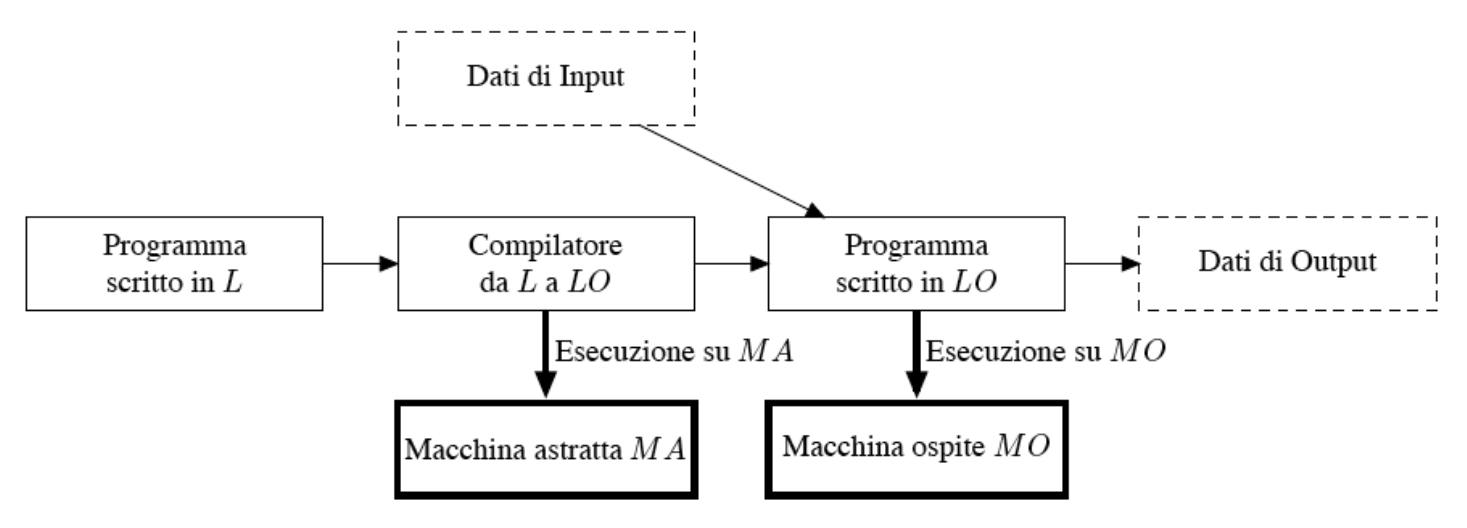
\includegraphics[scale=0.35]{media/compilatore}}
	  \caption{Struttura compilatore}
	\end{center}
\end{figure}

\begin{figure}[h!]
	\begin{center}
	  \fbox{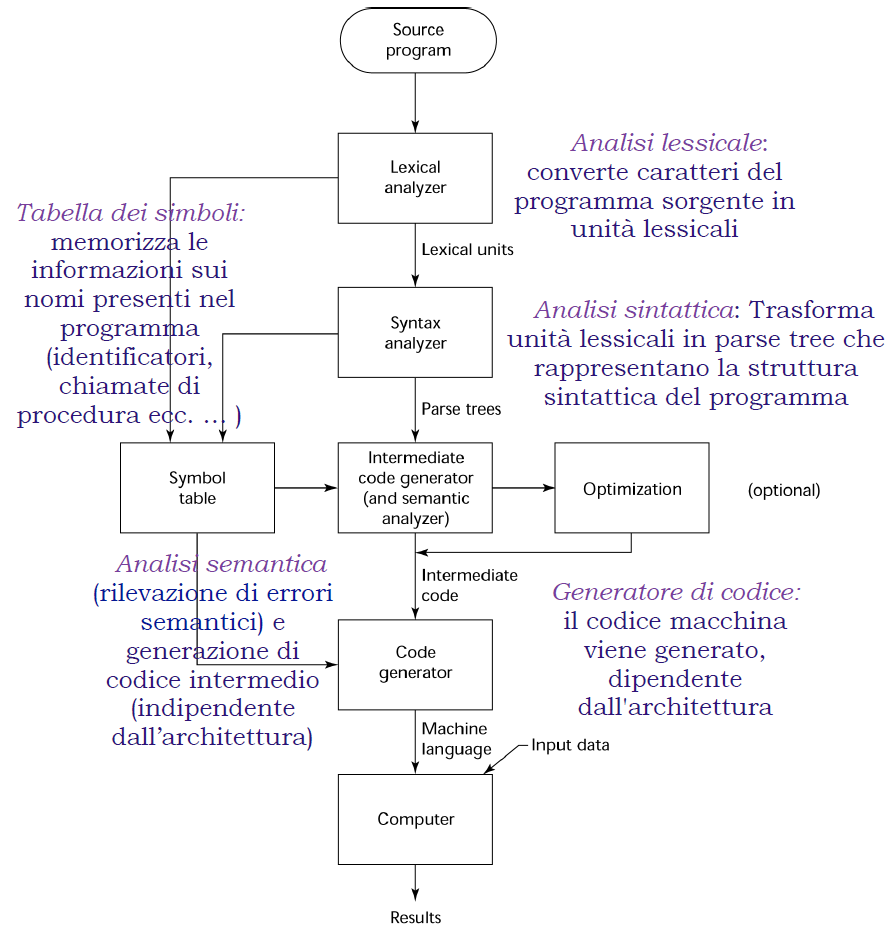
\includegraphics[scale=0.6]{media/struttura_compilatore}}
	  \caption{Flusso di esecuzione compilatore}
	\end{center}
\end{figure}

\clearpage

\subsection{Interprete vs Compilatore vs Ibrido}
\begin{itemize}
 \item \textbf{Interpretazione pura}: nessun costo di traduzione iniziale (comincio ad eseguire subito), esecuzione lenta per l'intepretazione di istruzioni ripetute, scarsa efficienza della macchina \texttt{ML}, buona flessibilità e portabilità, facilità di interazione a run-time e debugging (non si perde il legame tra il codice originale e quello interpretato)

 \item \textbf{Compilazione pura}: costo di traduzione iniziale sempre presente, esecuzione veloce (il risultato del compilatore è un programma tutto scritto in linguaggio macchina e ottimizzato), progettazione difficile, scarsa flessibilità, perdita di
informazione sulla struttura del programma sorgente (l'ottimizzazione rimuove e altera il codice originale, fare l'inverso è problematico)

 \item \textbf{Ibrido}: il linguaggio ad alto livello viene compilato in un linguaggio a più basso livello che poi viene interpretato (per esempio Java, dove il linguaggio intermedio è il Java ByteCode)
\end{itemize}

\begin{figure}[h!]
	\begin{center}
	  \fbox{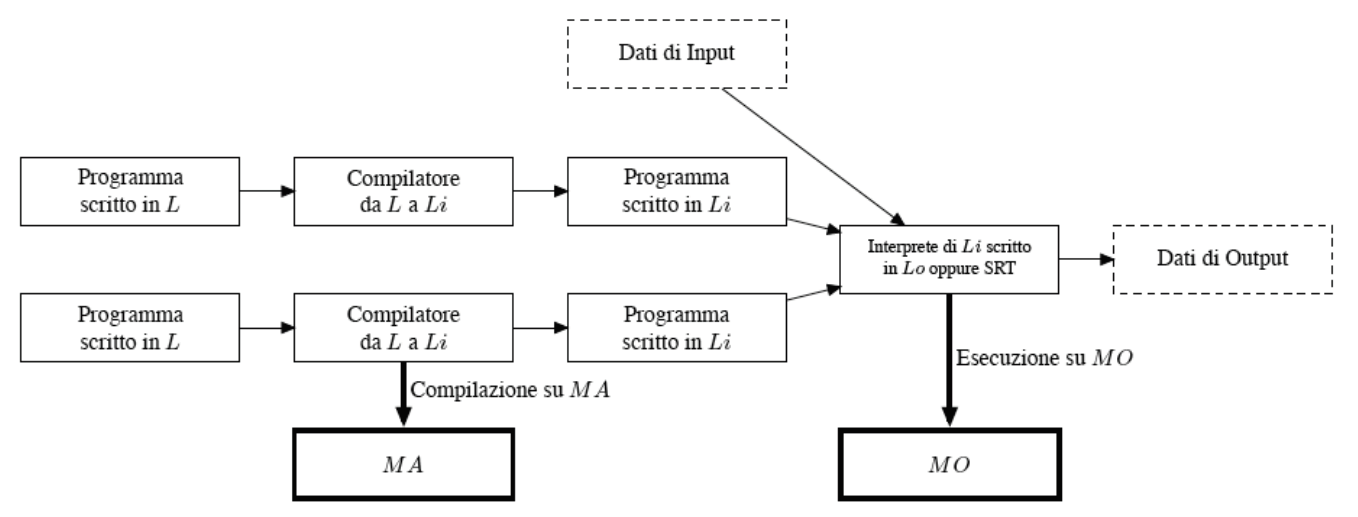
\includegraphics[scale=0.35]{media/soluzione_ibrida}}
	  \caption{Struttura della soluzione ibrida}
	\end{center}
\end{figure}

\begin{figure}[h!]
	\begin{center}
	  \fbox{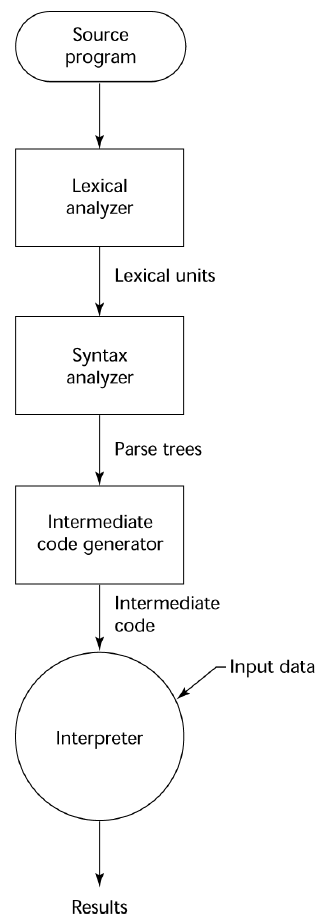
\includegraphics[scale=0.6]{media/struttura_soluzione_ibrida}}
	  \caption{Flusso di esecuzione della soluzione ibrida}
	\end{center}
\end{figure}

\clearpage

La compilazione deve tradurre un programma da un linguaggio ad un altro preservandone la semantica: dobbiamo avere la certezza che il programma compilato faccia esattamente quello che faceva il programma originale\slash sorgente, per questo un compilatore è uno strumento \textbf{più difficile da progettare} rispetto ad un interprete.

\subsection{Specializzatore}
Lo specializzatore valuta il programma su una parte dell' input, ottenendo un programma \textbf{specializzato rispetto a tale input} e, per questo, più efficiente su specifiche applicazioni. Intuitivamente, se abbiamo un programma in cui una parte dei dati in input è nota e non cambia, allora possiamo trasformare il programma in modo tale che le computazioni sulla parte nota dell'input siano state già svolte. Per questo si dice che lo specializzatore trasforma programmi, ovvero attua trasformazioni all'interno dello stesso linguaggio per migliorarne l'efficienza (nota anche come \textbf{Valutazione parziale}).

Esiste infatti un \textbf{legame semantico} tra interpreti e compilatori, ovvero \textbf{specializzando un interprete rispetto al programma otteniamo un compilatore} (\textbf{Proiezioni di Futamura}).

Quindi a partire da un interprete si garantisce l'esistenza di un compilatore, e in generale di trasformatori sintattici che preservano la semantica (ottimizzatori, offuscatori, \ldots).
%====================================
\clearpage
\section{Descrivere} \label{Descrivere}
Anche se artificiale, un PL è sempre un linguaggio, quindi deve essere descritto usando i noti strumenti della linguistica.
Gli aspetti che costituiscono un PL sono:
\begin{itemize}
\item \textbf{Sintassi}: le regole di formazione che permettono di costruire una frase corretta
\item \textbf{Semantica}: relazioni tra simboli e significato
\item \textbf{Pragmatica}: relazioni tra simboli, significato e utente (in quale modo frasi corrette e sensate vanno usate)
\item \textbf{Implementazione}: aspetti che hanno effetto sul funzionamento del linguaggio ma che
dipendono dalla macchina su cui il linguaggio viene eseguito (eseguire una frase corretta, rispettandone la semantica)
\end{itemize}
Semantica, pragmatica e implementazione sono elementi da studiare separatamente ma legati dalla sintassi in funzione della quale tutti sono definiti.

\subsection{Sintassi}
Le regole sintattiche del linguaggio specificano quali stringhe di caratteri sono legali nel linguaggio.

Nel dettaglio, la terminologia nella linguistica è la seguente:
\begin{itemize}
\item Una \textbf{parola} è una stringa di caratteri su un alfabeto
\item Una \textbf{frase} è una sequenza (ben formata) di parole
\item Un \textbf{linguaggio} è un insieme di frasi
\end{itemize}

Nell'ambito dei PL gli stessi concetti prendono nomi differenti, in particolare: 
\begin{itemize}
\item Le parole diventano \textbf{lessemi}.

Un lessema è una parola con significato specifico, nella grammatica corrisponde ad un terminale. È \textbf{l'unità minima sintattica}, ovvero quella a più basso livello di un PL (\texttt{*, sum, begin} \ldots). La loro specifica sintattica è separata dalla definizione del linguaggio, e come vedremo, solitamente descritta come stringhe di linguaggi regolari.

Ad esempio, in \texttt{index = 2;} , abbiamo tre lessemi: $(index, =, 2)$.

\item Le frasi diventano \textbf{token}.
 I token corrispondono agli elementi delle categorie sintattiche del PL, e nella grammatica corrispondono alle sequenze generate dai simboli non terminali (ad es. identificatore, comando, \ldots).

Ad esempio, \texttt{index = 2;} è un token (assegnamento\slash comando).
\item Il \textbf{programma} è una sequenza\slash composizione sequenziale di frasi ben formate
\end{itemize}

Il \textbf{linguaggio dei programmi}, e quindi gli strumenti formali che lo definiscono, costituiscono quello che chiamiamo \textbf{linguaggio di programmazione}. Questi concetti chiaramente non servono direttamente a chi usa il linguaggio, ma servono a chi lo deve implementare.

Il linguaggio dei lessemi è in generale sempre un linguaggio regolare, quindi riconosciuto da un automa a stati finiti.

Il linguaggio dei token, e quindi dei programmi, è in generale un linguaggio \textbf{Context-Free} (CF), quindi generato da una grammatica CF.
\subsection{Semantica}
Attribuisce un significato ad ogni frase sintatticamente corretta, ovvero ogni frase che rispetta le regole della grammatica.

Le tipologie di semantiche possono essere divise in tre macro classi:

\begin{itemize}
\item \textbf{Denotazionale, descrive funzionalità}: studia gli effetti dell'esecuzione, cerca proprietà del programma studiando proprietà della funzione calcolata
\item \textbf{Assiomatica, descrive proprietà}: serve per fare deduzioni logiche a partire da assiomi su parti del programma (dimostrazioni di correttezza)
\item \textbf{Operazionale, descrive trasformazioni di stato}:  si preoccupa di \textbf{come} i risultati finali vengono prodotti (permette l'implementazione di un interprete)

\end{itemize}

\subsection{Categorie sintattiche}
Possiamo dividere la sintassi di un PL in categorie, in base all'effetto che i costrutti di tale categoria hanno sullo stato della macchina.

Per far ciò dobbiamo prima introdurre i seguenti concetti:
\begin{itemize}
\item \textbf{Stato del programma}: insieme dei suoi ambienti e della sua memoria
\item \textbf{Ambiente} (environment): insieme di legami (bindings) tra identificatori e oggetti denotati, ovvero relazioni \textbf{nome-oggetto}
\item \textbf{Memoria} (store): insieme di effetti sugli identificatori (causati da assegnamenti), rappresenta la storia (non tutta) delle variazioni dei valori associati agli identificatori, fornisce un binding tra locazione e valore. Si noti che il concetto di memoria in questo senso è fortemente legato ai linguaggi imperativi.
\end{itemize}
\textbf{Importante}: è l'ambiente che mi dice in ogni istante a quale oggetto un nome si lega.

A questo punto possiamo identificare tre categorie sintattiche:
\begin{itemize}
\item \textbf{Espressioni}: generano valori. Vedi capitolo \ref{Espressioni}.
\item \textbf{Dichiarazioni}: creano legami. Vedi capitolo \ref{Dichiarazioni}.
\item \textbf{Comandi}: attuano trasformazioni di stato. Vedi capitolo \ref{Comandi}.
\end{itemize}
%====================================
\clearpage
\section{Espressioni} \label{Espressioni}
Una espressione è un oggetto sintattico che \textbf{denota un valore}, composto da operatori, operandi (che sono a loro volta altre espressioni), parentesi e, potenzialmente, chiamate a funzioni\slash procedure.

Le espressioni devono essere \textbf{valutate} per restituire un valore.

\textbf{Equivalenza}: Due espressioni sono equivalenti se vengono valutate nello stesso valore in tutti gli stati di computazione (anche eventuali side-effects devono essere gli stessi).

Come si caratterizzano:
\begin{itemize}
\item \textbf{Notazione}: specifica in che modo gli operandi e gli operatori vengono rappresentati e indica su quali operandi un operatore opera.
\item \textbf{Regole di precedenza} tra operatori, vedi sotto
\item \textbf{Regole di associatività} degli operatori, vedi sotto
\item \textbf{Ordine di valutazione degli operandi}
\item \textbf{Presenza di side-effects}: qualunque effetto che non consista puramente nella rappresentazione di valori
\item \textbf{Overloading degli operatori}: possono esistere operatori che hanno significato diverso a seconda del tipo degli operandi a cui sono applicati (\texttt{int+int} è una somma, \texttt{str+str} è una concatenazione)
\item \textbf{Espressioni con tipi misti}: alcuni PL permettono espressioni che combinano tipi diversi
\end{itemize}
Esistono tre tipi di notazione:
\begin{itemize}
\item \textbf{In-fissa}: \texttt{a+b}
\item \textbf{Pre-fissa} (polacca): \texttt{+ab}
\item \textbf{Post-fissa} (polacca inversa) : \texttt{ab+}
\end{itemize}
Pre\slash post-fissa non necessitano di regole di precedenza, associatività, parentesi. Permettono una \textbf{rappresentazione uniforme per qualunque arietà di operatori}.

\clearpage

Nel valutare le espressioni dobbiamo utilizzare diverse regole per togliere l'ambiguità sul come fare ciò:
\begin{itemize}
\item \textbf{Regole di precedenza}: Le regole di precedenza di un operatore per la valutazione di una espressione definisce l'ordine in cui operatori a diversi livelli di precedenza vengono valutati.

Tipiche regole di precedenza sono (in ordine decrescente): $(), */ , +-$.

Per esempio, in \texttt{a+b*c}, \texttt{+} e \texttt{*} sono a livelli diversi di precedenza: la regola scritta sopra mi dice che prima devo eseguire \texttt{*} e poi \texttt{+}

\item \textbf{Regole di associatività}: definiscono l'ordine con cui operatori allo stesso livello di precedenza vengono valutati. Tipiche regole di associatività sono associare da destra o da sinistra.
Per esempio, \texttt{a+b-c+d} dà risultati diversi se associata da destra o da sinistra
\end{itemize}

\textbf{Nota}: sia le regole di precedenza che associatività \textbf{possono essere sovrascritte usando le parentesi}.

\subsection{Valutazione}
Un PL deve rappresentare internamente le espressioni in modo da poterle manipolare.

Generalmente, la rappresentazione interna delle espressioni consiste in un albero rovesciato, detto \textbf{Abstract Syntax Tree}, dove \textbf{i nodi interni sono operatori} mentre le \textbf{foglie sono valori}, ovvero gli operandi elementari. Ogni nodo interno ha per figli gli alberi che rappresentano le espressioni a cui l'operatore si applica (operandi). L'albero fornisce quindi la struttura dell'espressione, ovvero elimina eventuali ambiguità legati a precedenze e associatività, ma non può dare informazioni riguardanti \textbf{l'ordine di valutazione dell'espressione} che invece è determinata dalla tipologia di visita che l'implementazione del PL effettua sull'albero.

Esistono due tipi di valutazione:
\begin{itemize}
\item \textbf{Valutazione lazy (short-circuit)}: valuta gli operandi solo quando necessario
\item \textbf{Valutazione eager}: valuta sempre tutti gli operandi
\end{itemize}
Per esempio, l'espressione \texttt{(a == 0 ? b : b/a)}, con valutazione lazy è sempre definita perché  \texttt{b/a} lo valuto solo se \texttt{a = 0}, mentre con valutazione eager l'espressione risulta non definita quando \texttt{a = 0}.

\textbf{Side effect}: modifiche di variabili non locali da parte di una funzione. Alcuni PL non permettono la definizione di tali funzioni.//TODO che ci fa qui sta def?
%====================================
\section{Dichiarazioni} \label{Dichiarazioni}
Una dichiarazione è un'oggetto sintattico che \textbf{denota richieste di modifica\slash creazione di legami} nome-oggetto, altera quindi gli ambienti.

Le dichiarazioni devono essere \textbf{elaborate} per attuare la creazione\barra trasformazione di legami.

Si noti che le modifiche agli ambienti sono trasformazioni \textbf{reversibili}, in quanto valgono esclusivamente all'interno del raggio di azione (scope) attuale dell'identificatore. Quindi è sufficiente aspettare la terminazione dell'ambiente in questione per far sì che le modifiche attuate al suo interno ``spariscano'' dal programma.

\textbf{Equivalenza}: Due dichiarazioni sono equivalenti se producono lo stesso ambiente (e la stessa memoria in caso di side effects) in tutti gli stati di computazione.

Un esempio di side-effect per le dichiarazioni è l'inizializzazione di una variabile: \texttt{int cont = 69} modifica la memoria (sarebbe compito dei Comandi), per questo l'equivalenza deve richiedere la stessa generazione di side-effect.

\subsection{Nome/Identificatore}
Entità (sequenza di caratteri) che \textbf{denota un oggetto} (procedura o cella di memoria).
Si noti come il legame tra i due non è \textit{assoluto}: lo stesso nome\barra identificatore può essere usato in contesti (scope) diversi per denotare oggetti diversi. Ovvero il suo binding può non essere lo stesso in ambienti diversi. La durata di un binding viene chiamata il suo ``\textbf{tempo di vita}''.
\subsection{Scelta degli identificatori}
L'uso degli identificatori ci permette di sostituire gli \textbf{indirizzi assoluti} della memoria con dei nomi, rendendo i programmi \textit{potenzialmente} molto più leggibli\slash scrivibili (astrazione). Per mantenere\slash sfruttare al meglio queste potenzialità la sequenza di caratteri usata come identificatore, oltre che rispettare limiti imposti dal PL (parole riservate, caratteri speciali, vincoli sulla lunghezza) deve essere scelta con cura dal programmatore.

Per esempio, una matricola alla prima lezione di Programmazione I potrebbe scrivere qualcosa tipo:
\begin{center}
\texttt{float var = 420.69;}
\end{center}

Un programmatore più esperto scriverebbe invece:
\begin{center}
\texttt{float numeroPreferito = 420.69}
\end{center}

Si noti come è di immediata comprensione cosa significhi il valore denotato dalla variabile, se associato ad un identificatore appropriato.
\subsection{Binding}
Associazione tra nome\slash identificatore e il suo significato. Fatto ciò, per tutto il tempo di vita del binding, si dice che il nome \textbf{denota} il significato.

Permettono astrazione sui dati e sul controllo a seconda dell'oggetto denotato.

\subsubsection{Tipi di binding}

\textbf{Scope di un binding}: definisce l'ambiente\slash i in cui si può usare un nome per denotare un'oggetto.

Distinguiamo i binding in base a \textbf{cosa} legano:
\begin{itemize}
\item \textbf{Nome-valore}: non modificabile (le costanti)
\item \textbf{Nome-locazione}: modificabile con assegnamento (puntatore)
\item \textbf{Locazione-valore}: modificabile con assegnamento (cambio contenuto di una variabile)
\end{itemize}
La relazione tra nome, valore e locazione viene approfondita nella sezione \ref{locazione}.

Distinguiamo i binding in base a \textbf{come} legano:
\begin{itemize}
\item \textbf{Binding statico}: detto anche \textbf{early binding}, viene effettuato a tempo di compilazione, le associazioni fatte (tipi delle varaibili in linguaggi fortemente tipizzati) rimangono invariate durante l'esecuzione del programma. Esecuzione veloce, programmazione poco flessibile, usa lo stack, indirizzi assoluti.
\item \textbf{Binding dinamico}: detto anche \textbf{late binding}, viene effettuato durante l'esecuzione, le associazioni fatte (locazione-valore) posono variare durante l'esecuzione. Esecuzione più lenta, programmazione flessibile, usa lo heap, indirizzi non assoluti.
\end{itemize}

\clearpage

\subsection{Semantica}
Il significato di una dichiarazione è essenzialmente un ambiente (insieme di legami).

\textbf{Termine chiuso}: termine in cui non ci sono identificatori liberi.

Quindi un programma è una frase chiusa se ogni occorrenza d'uso è preceduta da una occorrenza di definizione che stabilisce il significato dell'identificatore.

\textbf{Termine ground}: termine in cui non ci sono identificatori.

Chiaramente un termine ground non richiede un ambiente non avendo identificatori.

\textbf{Tipo}: determina l'insieme di valori (che condividono una certa proprietà strutturale) dotato di un insieme di operazioni definite per i valori di quel tipo. Esempi di tipo sono \texttt{int, float, bool, string, char,}\ldots.

\subsubsection{Type binding}
Il binding tra nome e tipo può essere di due tipi:
\begin{itemize}
\item \textbf{Statico}: non può cambiare durante l'esecuzione del programma (C, C++, Java)
\item \textbf{Dinamico} (solo per linguaggi interpretati): può cambiare durante l'esecuzione (Python, JS), costi maggiori di implementazione, più flessibile
\end{itemize}

\subsection{Semantica statica e dinamica}
In seguito all'introduzione dei tipi di dato, dividiamo la semantica in due:
\begin{itemize}
\item \textbf{Semantica statica}: per la creazione di legami di tipo e per la verifica della corretta forma degli elementi di un programma.

Controlla la forma e permette di controllare quelli che abbiamo chiamato vincoli contestuali. I legami di tipo sono raccolti nel così detto \textbf{ambiente statico}, creato esclusivamente dalla semantica statica delle dichiarazioni.
\item \textbf{Semantica dinamica}: per la valutazione delle espressioni, l'elaborazione delle dichiarazioni e l'esecuzione dei comandi.

Permette di creare e modificare i legami con gli oggetti denotati (valori, locazioni, \ldots). Questi legami sono quelli che formano il così detto \textbf{ambiente dinamico}, il quale viene creato e modificato durante l'elaborazione delle dichiarazioni e l'esecuzione dei comandi
\end{itemize}

\subsubsection{Compatibilità di ambienti}

Sia $\rho:V$ un ambiente dinamico e $\Delta:V$ un ambiente statico con $V\subseteq_f Id$.

Gli ambienti $\rho$ e $\Delta$, sono compatibili (scritto $\rho:\Delta$) se e soltanto se:

\begin{center}
$\forall id \in V . (\Delta(id) = \tau \wedge \rho(id) \in \rho)$
\end{center}

Dove $V$ è l'insieme degli identificatori.

A parole, un ambiente statico e uno dinamico sono compatibili se parlano in modo coerente degli stessi identificatori, ovvero, se l’ambiente statico stabilisce che una certa espressione ha tipo $\tau$, allora la semantica dinamica deve arrivare ad associare all’identificatore un valore contenuto nel tipo $\tau$.
%====================================
\section{Comandi} \label{Comandi}
Un comando è un'oggetto sintattico che \textbf{denota la richiesta di modifica della memoria} tramite \textbf{assegnamento}.

I comandi devono essere \textbf{eseguiti} e rappresentano funzioni di trasformazione.

Si noti che queste ultime sono \textbf{irreversibili}, nel senso che per tornare allo stato precedente di memoria devo eseguire un altro comando.

\textbf{Equivalenza}: Due comandi sono equivalenti se per ogni stato (memoria) in input producono lo stesso stato (memoria) in output.

Essendo i comandi trasformatori di memorie, possiamo dire che sono funzioni da memorie a memorie.

Un esempio di side-effect per i comandi è la generazione di valori e creazione legami, per questo l'equivalenza richiedere l'equivalenza di side-effect.

I comandi sono tipici del paradigma imperativo, non essendo presenti in linguaggi logici o funzionali puri.
\subsection{Locazione}\label{locazione}
Per gestire gli identificatori variabili (le \textit{variabili}, appunto) abbiamo bisogno di raffinare lo stato: non va bene astrarre la cella di memoria solo con un nome (in un certo senso astrae troppo).

Introduciamo quindi il concetto di \textbf{locazione}, che si pone tra l'identificatore e il valore da esso denotato.

\begin{center}
\textbf{Identificatore $\rightarrow$ Locazione $\rightarrow$ Valore}
\end{center}

Ovvero, medianto l'uso di un identificatore denotiamo una locazione (cella) di memoria, la quale contiene un valore.

In questo modo, con lo stesso identificatore, possiamo denotare locazioni diverse, in \textbf{differenti momenti dell'esecuzione}.

\textbf{Alias}: vengono così chiamati gli identificatori che denotano la stessa locazione nello stesso istante di esecuzione.

Si noti come una locazione non deve necessariamente essere riferibile per sempre durante l'esecuzione, essa infatti ha un tempo di vita determinato dallo \textbf{scope della dichiarazione}. Il modo in cui si rilascia la locazione, ovvero la perdita del legame nome-locazione, determina la \textbf{reversibilità dei cambiamenti}: se il rilascio è \textbf{implicito} (automatico) il cambiamento è reversibile, mentre se è \textbf{esplicito} (allocazione dinamica) il cambiamento diventa non reversibile.

\subsection{Costanti e variabili}
La differenza tra costanti e variabili è:
\begin{itemize}
\item \textbf{Costanti}: binding tra l'identificatore e il un valore
\item \textbf{Variabili}: binding tra l'identificatore e una locazione, la quale contiene un valore
\end{itemize}
Notiamo che le variabili quindi, oltre ad essere caratterizzate da nome\slash identificatore, tipo e valore come lo sono le costanti, sono caratterizzate anche da:
\begin{itemize}
\item \textbf{indirizzo\slash locazione}: consiste nell'oggetto denotabile legato all'identificatore della variabile.
\item \textbf{scope}: il range dei comandi a cui la variabile è visibile, ovvero dove è visibile la sua dichiarazione
\item \textbf{tempo di vita}: ovvero tempo in cui il binding con la locazione è attivo
\end{itemize}
\subsection{Strutture di controllo: selettori}
Il controllo dell'esecuzione avviene grazie a delle strutture di controllo, ovvero comandi che specificano l'ordine con cui le modifiche (assegnamenti) devono essere eseguite, oltre che alternative e ripetizioni di comandi.

La prima classe di strutture di controllo sono i \textbf{comandi di selezione}, ovvero comandi che permettono di per scegliere tra due o più cammini di esecuzione, rispettivamente \texttt{if} e \texttt{switch} statement.

\subsection{Strutture di controllo: composizione}
La composizione sequenziale, denotata dal \texttt{;} permette di specificare in modo diretto la composizione di comandi denotando il fatto che il comando a destra del simbolo di composizione inizia dopo che il comando a sinistra ha completato l'esecuzione.

\subsection{Strutture di controllo: comandi iterativi}
Per ottenere linguaggi \textbf{Turing completi} abbiamo bisogno di inserire nel linguaggio la possibilità di ripetere comandi. L'esecuzione ripetuta di un comando si ottiene mediante \textbf{iterazione} o \textbf{ricorsione}.

Esistono due tipi di iterazione:
\begin{itemize}
\item \textbf{Indeterminata}: realizzata mediante ciclo \textbf{while}, dove la condizione di iterazione è una espressione booleana, il cui valore è controllato ad ogni passo, non è noto a priori il numero di iterazioni da eseguire
\item \textbf{Determinata}: realizzata mediante ciclo \textbf{for}, dove la condizione di iterazione è una espressione numerica, è noto a priori il numero di iterazioni da eseguire
\end{itemize}


\textbf{Note:}
\begin{itemize}
\item Nel ciclo while, bisogna specificare se eseguire il \textbf{pre-test}, ovvero il ciclo \textbf{while-do}, il quale prima controlla che l'espressione di controllo si vera e poi eseguire il corpo del ciclo, o il \textbf{post-test}, ovvero il ciclo \textbf{do-while}, il quale prima esegue il corpo del ciclo e poi valuta l'espresione per decidere se iterare ancora.
\item Nel ciclo for, si può rendere la variabile di iterazioni modificabile all'interno del ciclo. Inoltre si può scegliere di valutare l'espressione di controllo ad inizio ciclo o ad ogni iterazione.
\end{itemize}

\subsection{Blocchi: integrazione di ambienti e memorie}
Un blocco è una \textbf{regione testuale} che può contenere dichiarazioni locali e comandi. Serve inoltre per ``delimitare'' un ambiente, ovvero le associazioni dichiarate localmente assieme a quelle globali. 

L'uso dei blocchi permette una gestione locale dei nomi e aumenta la chiarezza della struttura del codice.

Permettono la ricorsione, e permettono l'esecuzione di comandi in ambienti modificati.

Solitamente sono identificati da \textbf{delimitatori} (es. parentesi) che ne determinano lo scope.

I blocchi non possono essere parzialmente sovrapposti, ovvero o sono \textbf{disgiunti} o sono \textbf{annidati}.

\textbf{Regola di visibilità}: una dichiarazione locale ad un blocco è visibile in quel blocco e in tutti i blocchi in esso annidati, a meno che non intervenga in tali blocchi una nuova dichiarazione dello stesso nome, la quale nasconde\slash maschera, la precedente.

Tanti blocchi annidati possono creare problemi di leggibilità, ma possono anche rendere più complesso il recupero del giusto riferimento, e infine possono complicare il debugging, ma vengono usati per permettere ai programmatori di usare i propri nomi, indipendentemente da altre porzioni di codice dentro al quale fanno eseguire il proprio.

Concludendo, quando si entra in un blocco si creano associazioni locali, se sono presenti dichiarazioni, e si disattivano le sovrapposizioni (associazioni precedenti con lo stesso nome), all'uscita si distruggono le associazioni locali e si riattivano quelle al livello superiore.

\subsection{Blocchi: tipi di ambienti}
Lo scope di una variabile (definita) è quindi il range di comandi ai quali è visibile.
\begin{itemize}
\item \textbf{Ambiente locale}: associazioni create dentro il blocco corrente
\item \textbf{Ambiente non locale}: associazioni fatte in altri blocchi, di cui alcune immediatamente visibili come le variabili globali, altre da determinate, vedi sezione  \ref{regoleScoping}
\item \textbf{Ambiente globale}: quella parte di ambiente non locale relativo alle associazioni comuni a tutti i blocchi, ovvero dichiarazioni esplicite di variabili globali e associazioni esportate da moduli
\end{itemize}

\subsection{Blocchi: tempo di vita}
Scope e tempo di vita sono concetti molto vicini, ma di natura diversa:
\begin{itemize}
\item Lo scope (statico) è un \textbf{concetto spaziale}, definito a tempo di \textbf{compilazione}, ovvero in quale sezione di codice posso usare quell'identificatore
\item Il tempo di vita (lifetime) è un \textbf{concetto temporale}, definito a tempo di \textbf{esecuzione}
\end{itemize}

\section{Procedure}
L'uso delle procedure permette la così detta \textbf{astrazione del controllo}.

Astrarre significa nascondere dettagli concreti facendo emergere con più
chiarezza concetti comuni.

Le procedure sono anche uno strumento che permette la
\textbf{scomposizione di un problema in sottoproblemi}, permettendo così di gestirne la
complessità. La soluzione globale si ottiene combinando in modo opportuno le
soluzioni dei sottoproblemi.

Le motivazioni che stanno dietro al processo di astrazione sono:
\begin{itemize}
\item maggiore leggibilità del codice
\item utilizzo ripetuto delle stesse espressioni o gruppi di comandi
\item riduzione delle possibilità di errore, ovvero abbreviare la scrittura di programmi che contengono sequenze ripetute di comandi uguali che possono differire sull'input
\end{itemize}

Parte essenziale del processo di astrazione è dare un nome al raggruppamento, il quale permette di riferirsi all'astrazione senza conoscerne i dettagli ma solo le caratteristiche di interesse che ne hanno determinato il raggruppamento.

Astrazione del controllo significa quindi legare negli ambienti una sequenza di comandi, detta \textbf{corpo della procedura}, ad un identificatore, ovvero il \textbf{nome} della procedura.

Aggiungendo i parametri al nome e corpo della procedura possiamo eseguire la stessa computazione in contesti differenti.

Nome e parametri formano l'\textbf{interfaccia dell'astrazione} o \textbf{firma della procedura}, ovvero tutto ciò che è necessario conoscere per poter usare correttamente la procedura, mentre il
corpo è proprio l'informazione che viene astratta.

Quando viene chiamata una procedura il programma chiamante viene sospeso durante l'esecuzione del programma chiamato, e riprende quando quest'ultimo ha terminato.

\textbf{Sottoprogramma}: chiamato anche funzione o procedura (la prima ritorna un valore, la seconda no), è una porzione di
codice identificato da un nome, dotato di un ambiente locale proprio e capace di scambiare informazioni con il resto del codice mediante parametri e valori di ritorno.

\textbf{Ambiente di riferimento di un comando}: è la collezione di tutte le associazioni nome-oggetto visibili al comando.

\subsubsection{Ambiente di riferimento di una procedura}
L'ambiente di riferimento di una procedura è determinato in modi diversi a seconda della situazione:

\begin{itemize}
\item Quando una funzione usa solo nomi definiti nell'ambiente locale, non c'è bisogno di risolvere nulla, in quanto i valori di quelle variabili sono esattamente quelli definiti nel suo corpo.

\item Quando una funzione usa nomi non locali, allora bisogna risolvere tale nome con le \textbf{Regole di Scoping}, statico o dinamico che sia a seconda del PL (vedi \ref{regoleScoping})

\item Quando una funzione usa nomi non locali e viene passata come parametro ad un'altra funzione, in caso di scoping statico non ci sono dubbi in quanto si va a guardare l'ambiente di definizione, mentre nel caso di scoping dinamico bisogna scegliere se usare l'ambiente in cui la funzione è stata ``chiamata'' per essere passata come parametro e l'ambiente della funzione che effetivamente esegue la funzione passatagli come parametro, bisogna introdurre quindi le \textbf{Politiche di Binding} (vedi \ref{politicheBinding})
\end{itemize}

\textbf{Conseguenza}: nel caso cui le funzioni di un programma utilizzino solo nomi locali e non siano mai passate come parametri non serve parlare né di scoping né di binding.

\subsection{Allocazione della memoria}
Un concetto fortemente legato all’uso delle procedure è l’allocazione della memoria, ovvero come vengono allocati gli oggetti e dove vengono risolti i riferimenti (non locali).

Esistono due meccanismi di allocazione della memoria:
\begin{itemize}
\item \textbf{Statica}: memoria allocata a tempo di compilazione, prima dell'inizio dell'esecuzione  i dati del programma vengono disposti in opportune zone di memoria dove rimangono fino alla fine.

Molto efficiente, meno libertà di programmazione perché impedisce la ricorsione (non so a priori quante chiamate farò, ovvero quanta memoria mi servirà).

I PL moderni non sono mai completamente ad allocazione statica, tranne per alcuni aspetti come le costanti e l'uso di alcune keyword (\textit{static} in Java).

\item \textbf{Dinamica}: memoria allocata a tempo di esecuzione, si usano delle strutture dinamiche che durante l'esecuzione vengono continuamente allocate e deallocate. In particolare, le strutture tipicamente usate sono due: \textbf{Pila} (stack), dove gli oggetti vengono allocati con politica LIFO e lo \textbf{Heap}, dove gli oggetti possono essere allocati e deallocati in qualsiasi momento.

Fa uso degli RdA per memorizzare le varie chiamate ricorsive, vedi capitolo \ref{RdA}.
\end{itemize}
\subsection{Record di attivazione}\label{RdA}
Per ogni procedura chiamata viene salvato sullo stack un \textbf{record di attivazione} (\textbf{RdA}), ovvero una struttura dati che memorizza le informazioni necessarie per la gestione della procedura. L'RdA viene usato tramite un puntatore chiamato \textbf{SP} (stack pointer) che punta all'RdA attivo (ultima funzione chiamata, quella in esecuzione). 

Un Rda è composto da:
\begin{itemize}
\item \textbf{Puntatore di Catena Dinamica}: puntatore all'RdA del blocco che ha chiamato il blocco in esecuzione
\item \textbf{Puntatore di Catena Statica}: puntatore all'RdA del blocco che contiene sintatticamente il testo del blocco in esecuzione.
\item \textbf{Indirizzo di ritorno}: punta all'istruzione da eseguire dopo il ritorno
\item \textbf{Indirizzo del risultato}: punta alla locazione di memoria dove depositare il risultato della procedura (può non esserci)
\item \textbf{Parametri}: i parametri passati alla funzione
\item \textbf{Risultati intermedi}: quelli ottenuti dall'esecuzione della procedura
\end{itemize}
Dentro gli RdA è possibile accedere alle variabili locali attraverso il loro offset dall'inizio del RdA. Questo offset è chiamato anche \textbf{local offset} della variabile locale, che può essere determinato a tempo di compilazione.

\subsection{Semantica delle chiamate}
La semantica della chiamata ad un sottoprogramma deve essere specificata sotto diversi punti di vista:
\begin{itemize}
\item Metodi di passaggio di parametri
\item Allocazione dinamica sullo stack delle variabili locali
\item Salvataggio dello stato di esecuzione del programma chiamante
\item Trasferimento del controllo e preparazione del ritorno
\item Se è supportato l'annidamento di sottoprogrammi, deve essere gestito l'accesso a variabili non locali
\end{itemize}
In queste fasi quindi abbiamo la modifica del program counter del programma, l'allocazione dell'RdA e la modifica del puntatore allo stack. Analogamente, anche la semantica del ritorno da un sottoprogramma si basa sull'implementazione di varie fasi:
\begin{itemize}
\item Deallocazione dello stack per le variabili non locali
\item Recupero dello stato di esecuzione del chiamante
\item Ritorno del controllo al chiamante
\end{itemize}
L'operazione principale nel ritorno è il ripristino del program counter.

\subsection{Regole di scoping} \label{regoleScoping}
Quando le procedure fanno riferimento a variabili non locali (non definite nel loro corpo), per capire a quale variabile non locale andare a riferirsi, devono fare uso delle regole di scoping.
\subsubsection{Scope statico}
I nomi non locali sono risolti a tempo di compilazione, utilizzando l'ambiente valido al momento della definizione di tale nome, l'implementazione che vediamo è:
\begin{itemize}
\item \textbf{Catena statica (CS)}: lista di link statici che collegano ogni RdA al proprio antenato
\end{itemize}
Per risolvere i riferimenti di una variabile \texttt{x} in un sottoprogramma \texttt{P}, possiamo determinare, dalle informazioni note staticamente, qual'è il sottoprogramma \texttt{D} più vicino (nella catena di annidamento) che definisce \texttt{x}. Quindi possiamo calcolare il numero di volte \texttt{N} di cui risalire la catena statica come: \texttt{N = Sd(P) - Sd(D)}.

Si noti come lo scope statico garantisca \textbf{l'indipendenza del risultato} della procedura dalla sua posizione nel codice.

Il link statico di una procedura \texttt{P} che viene chiamata, si determina come: \texttt{Sd(chiamante) - Sd(P) + 1}.

\subsubsection{Scope dinamico}
I nomi non locali sono risolti a tempo di esecuzione, utilizzando l'ambiente valido al momento della chiamata della procedura che usa tale nome: l'associazione nomi-oggetti dipende dal flusso dell'esecuzione.

La regola generale è semplice: l'associazione corrente per un nome è quella determinata per ultima durante l'esecuzione.
\begin{itemize}
\item \textbf{Deep Access}: le variabili non locali vengono trovate cercando negli RdA lungo la catena dinamica
\item \textbf{Shallow Access}: si pongono le variabili locali in strutture dati centrali, ovvero si costruisce uno stack per ogni nome di variabile e si mantiene una tabella centrale con una entry per ogni nome di variabile
\end{itemize}
Un'implementazione dello Shallow Access è la \textbf{Tabella Centrale dei Riferimenti} (\textbf{CRT}).
Ogni entry della tabella rappresenta una variabile, il quale punta alla lista di elementi che rappresentano i vari ambienti dove la variabile è definita.

Quindi per ogni identificatore usato nel programma, l'ambiente valido in un qualunque momento per quell'identificatore è quello puntato dal primo elemento della lista (l'ultimo aggiunto).

La CRT viene aggiornata ogni volta che viene aggiunto e tolto un RdA dallo stack.

L'accesso è in tempo costante anche se con costi di gestione di ingresso\slash uscita.

La collezione di link dinamici nello stack, validi in ogni punto di esecuzione, è chiamata \textbf{catena dinamica}, o \textbf{catena delle chiamate}.

\begin{figure}[h!]
	\begin{center}
	  \fbox{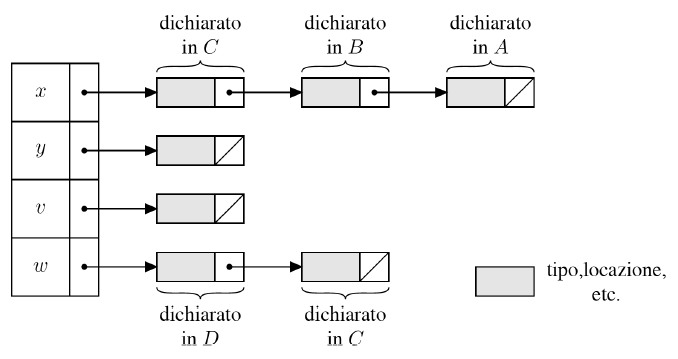
\includegraphics[scale=0.81]{media/CRT}}
	\end{center}
\end{figure}

\textbf{Nota}: lo scope statico (Python, Java, C) è più difficile da implementare ma più efficiente del dinamico (Perl).

\clearpage

\subsubsection{Ambiente di riferimento per un nome}
Dato un nome, il suo l'ambiente di riferimento è determinato dalle regole di:

\begin{itemize}
\item \textbf{Scoping}
\item \textbf{Passaggio dei parametri}
\item \textbf{Binding}: da considerare solo nei linguaggi che permettono di passare procedure come parametri, in tal caso devo scegliere tra ambiente di definizione, ambiente di passaggio come parametro e ambiente di esecuzione
\item \textbf{Regole specifiche del linguaggio}: riguardano la relazione \textbf{visibilità-posizione}, alcuni linguaggi permetto di usare un nome anche prima di dichiararlo, basta che sia dichiarato nello stesso blocco prima o poi
\end{itemize}

\subsection{Parametri}
I parametri permettono l'astrazione di tante computazioni simili a nomi comuni. Formano così \textbf{l'interfaccia dell'astrazione}.

Possono essere di tipo:
\begin{itemize}
\item \textbf{Formale}: variabile nella firma della procedura, usata per la definizione\slash dichiarazione della procedura
\item \textbf{Attuale}: valore o indirizzo usato per istanziare il parametro formale corrispondente
\end{itemize}
Al termine di una procedura il \textbf{\textit{valore}} del parametro formale viene perso.

Il binding tra parametro formale e attuale può essere:
\begin{itemize}
\item \textbf{Posizionale}: il primo parametro attuale è legato al primo formale e così via, sicuro ed effettivo
\item \textbf{Keyword}: il nome del parametro formale a cui un attuale si riferisce è specificato insieme all'attuale al momento della chiamata. Il vantaggio è che i parametri possono apparire in qualunque ordine, evitando errori di corrispondenza, lo svantaggio è che l'utente deve conoscere i nomi dei parametri formali.
\end{itemize}

\textbf{Nota}: alcuni linguaggi ammettono parametri attuali di default nel caso in cui non vengano passati parametri attuali.

Nella creazione del legame tra parametri attuali e formali si possono usare vari modelli sia di comunicazione che concettuali.

\subsection{Modelli di comunicazione}
Specificano in che direzione si sposta l'informazione tra chiamante e chiamato
\begin{itemize}
\item \textbf{In-mode}: l'informazione viaggia in un'unica direzione, dal chiamante al chiamato mediante l'uso dei parametri.
\item \textbf{Out-mode}: l'informazione viaggia in un'unica direzione dal chiamato al chiamante sempre principalmente mediante l'uso dei parametri (in C\# un parametro dichiarato \texttt{out} viene ritornato al chiamante). Si può inoltre ritornare un valore al chiamante tramite la keyword \texttt{return}.
\item \textbf{Inout-mode}: l'informazione viaggia in entrambe le direzioni tra chiamante e chiamato mediante parametri e valore di ritorno.
\end{itemize}

\textbf{Nota:} In tutti e tre i casi, il chiamante e chiamato possono comunque comunicare mediante le variabili visibili ad entrambi.

\begin{figure}[h!]
	\begin{center}
	  \fbox{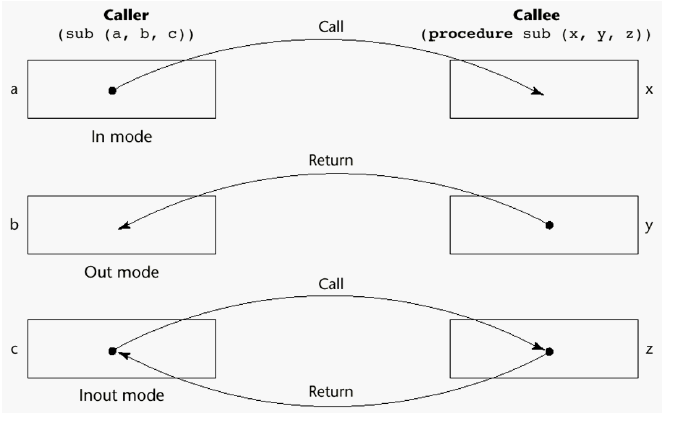
\includegraphics[scale=0.81]{media/modelli_comunicazione_procedure}}
	\end{center}
\end{figure}

\clearpage

\subsection{Modelli di concettuali}
Specificano come fisicamente il valore si sposta tra chiamante e chiamato.

\subsubsection{Passaggio per valore}
Usa la \textbf{in-mode}, richiede la valutazione completa del parametro a priori. Questo implica che il parametro attuale è una espressione (\texttt{r-value}) mentre il parametro formale deve essere un riferimento (\texttt{l-value}). Al momento della chiamata l'ambiente locale della procedura viene esteso con l'associazione tra attuali e formali visti come variabili locali, ovvero i parametri formali vengono \textbf{inizializzati} con il valore degli attuali. Quindi il passaggio consiste in una semplice inizializzazione, le modifiche future dei formali non si riflettono negli attuali. Non c'è un ritorno di informazione al chiamante mediante i parametri, quindi non generano \textbf{side-effects}.

Il vantaggio principale è la velocità di passaggio per valori scalari, lo svantaggio principale è il costo in spazio quando si passano valori di grandi dimensioni.

\subsubsection{Passaggio per risultato}
Usa la \textbf{out-mode}: nessun valore è passato alla procedura, ritorna un valore

\subsubsection{Passaggio per valore-risultato}
Usa la \textbf{in-out-mode}: combina il passaggio per valore con il passaggio per risultato

\subsubsection{Passaggio per riferiemento}
Usa la \textbf{in-out-mode}: viene passato un cammino di accesso al parametro attuale (puntatore).

I parametri attuali devono quindi essere \texttt{l-value} (riferimenti), e viene assegnato ai formali il riferimento dell'attuale. Durante l'esecuzione tutti i riferimenti al valore (\texttt{r-value}) del formale sono riferimenti al valore (\texttt{r-value}) dell'attuale e tutti cambiamenti del formale sono cambiamenti dell'attuale perché entrambi puntano alla stessa locazione.

L'implementazione è efficiente sia in tempo che in spazio, perché \textbf{non esegue copie}, ma crea alias.

\subsection{Funzioni di ordine superiore}
Alcuni linguaggi permettono di passare funzioni come argomenti di procedure e di restituire funzioni come risultato di esse. In entrambi i casi ci dobbiamo porre il problema di come gestire l'ambiente non locale della funzione. Il caso più semplice è il passaggio di funzioni come argomento, ovvero è sufficiente considerare un puntatore al record di attivazione all'interno della pila, ovvero si passa un valore detto \textbf{chiusura}, che è l'associazione tra nome e corpo della procedura. Il caso più complicato si ha quando la funzione viene ritornata da una procedura, ovvero bisogna mantenere il record di attivazione della funzione restituita: purtroppo in tal caso la pila non funziona!

Quando si hanno funzioni di ordine superiore che fanno riferimento ad \textbf{ambienti non locali}, per risolvere i nomi non è più sufficiente usare le regole di scoping, ma dobbiamo anche introdurre le \textbf{politiche di binding}.

\subsubsection{Politiche di binding} \label{politicheBinding}
Quando una procedura viene passata come parametro dobbiamo stabilire una politica di binding per capire quale ambiente non locale usare.

Con scope statico non ci sono dubbi: l'ambiente da usare è sempre quello valido al momento della definizione della funzione passata come parametro.
Con scope dinamico invece, dobbiamo decidere se risolvere i riferimenti nell'ambiente dove la funzione è \textbf{passata come parametro} (riga 19 esempio sotto), oppure l'ambiente dove effetivamente la funzione viene \textbf{chiamata per essere eseguita} (riga 14).

Distinguiamo quale scegliere tra i due con la seguente terminologia:
\begin{itemize}
\item \textbf{Deep binding}: ambiente valido al momento della creazione del legame tra il parametro attuale e il parametro formale, ovvero quando la funzione viene passata come parametro
\item \textbf{Shallow binding}: ambiente valido al momento della chiamata di quello che era il parametro attuale attraverso il parametro formale
\end{itemize}

\lstinputlisting[language=C]{./media/shallow_deep_binding.txt}

\clearpage

\subsection{Funzioni Ricorsive}
La ricorsione è un metodo alternativo all'iterazione per ottenere il potere espressivo delle MdT. Le due differiscono nell'utilizzo della memoria, ovvero la ricorsione crea un nuovo RdA per ogni chiamata ricorsiva, l'iterazione invece lavora sempre sullo stesso RdA.


Una funzione si dice ricorsiva se viene definita in termini di sè stessa. Le funzioni ricorsive derivano direttamente dalle definizioni per induzione, in cui un concetto è definito in termini di sè stesso ma su dati più piccoli.

Osserviamo comunque che ricorsione e induzione sono due concetti \textbf{molto diversi}. Una definizione induttiva (concetto matematico) è \textbf{sempre ben fondata}, ovvero arriva sempre ad una \textbf{base della definizione}, altrimenti non si potrebbe proprio parlare di induzione. Invece un programma ricorsivo (concetto informatico) \textbf{può divergere}, ovvero potrebbe \textbf{non terminare}, oppure potrebbe non definire nulla di significativo.

La ricorsione è possibile in ogni linguaggio che permette:
\begin{itemize}
\item Funzioni (procedure) che possono chiamare sè stesse
\item \textbf{Allocazione dinamica}, in quanto il compilatore non può sapere quanta memoria allocare per la catena di chiamate ricorsive, la cui lunghezza non è definita a priori
\end{itemize}
\textbf{Nota}: Ogni programma ricorsivo può essere tradotto in uno equivalente iterativo e viceversa, anche se la ricorsione è più naturale con linguaggi funzionali e logici, mentre l'iterazione è più naturale con linguaggi imperativi.

Esiste la possibilità di scrivere la ricorsione in modo efficiente nella gestione della memoria, riutilizzando sempre lo stesso RdA. Questa si dice \textbf{ricorsione in coda} (vedi \ref{ricorsione di coda}), e non è supportata da tutti linguaggi.
\subsection{Ricorsione di coda}\label{ricorsione di coda}
Una funzione ricorsiva si dice \textbf{ricorsiva in coda} (tail recursive) se contiene \textbf{solo} chiamate ricorsive in coda.

Una chiamata di \texttt{g} in \texttt{f} di si dice in coda (tail call) se \texttt{f} restituisce il valore restituito da \texttt{g} \textbf{senza ulteriori computazioni}.

Una funzione ricorsiva in coda permette una \textbf{gestione statica della memoria}, in quanto necessita di allocare un solo RdA perché tutte le chiamate possono essere sovrascritte, non avendo bisogno di ritornare valori che devono essere ulteriormente elaborati dal chiamante.

La trasformazione avviene definendo una funzione non ricorsiva, che chiama una funzione ausiliaria ricorsiva in coda, a cui viene aggiunto, rispetto alla versione ricorsiva non in coda, un parametro (nell'esempio sotto è \texttt{res}) che raccoglie ad ogni iterazione il \textbf{risultato parziale}, in modo da non dover elaborare valori dopo le chiamate ricorsive.

\begin{figure}[h!]
	\begin{center}
	  \fbox{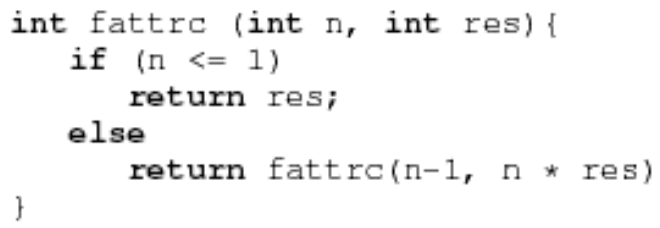
\includegraphics[scale=0.5]{media/fatt_tail_recursive}}
	  \caption{Fattoriale implementato con la ricorsione in coda}
	\end{center}
\end{figure}

\textbf{Note}:
\begin{itemize}
\item In generale, la ricorsione è meno efficiente dell'iterazione per il maggiore utilizzo di memoria, in termini di tempo di esecuzione invece, dipende dal codice.
\item In generale, ogni funzione ricorsiva può essere trasformata in una ricorsiva in coda.
\item La ricorsione costruisce il risultato \textbf{top-down}, mentre la ricorsione di coda lo costruisce \textbf{bottom-up}.
\item Il PL non può riconoscere da solo che l'algorimto ricorsivo è ricorsivo di coda, pertanto deve essere il programmatore a specificarlo tramite keywords
\end{itemize}

\section{Paradigmi di programmazione}
Un paradigma di programmazione rappresenta uno \textbf{stile fondamentale di programmazione}.

Diversi paradigmi si differenziano tra loro per diverse astrazioni e concetti messi a disposizione dell'utente per descrivere, tramite il codice, la realtà che si vuole rappresentare.

\subsection{Imperativo}
Un PL si dice Imperativo se si basa sulla Macchina di Von Neumann, ovvero usa l'astrazione della cella di memoria in variabile come costrutto principale per rappresentare e manipolare dati in memoria.

\subsection{Orientato agli oggetti}
Un PL si dice Orientato agli Oggetti se \textbf{estende}, quindi implementa, il paradigma Imperativo aggiungendo supporto per gli oggetti.


Un Oggetto è una collezione di dati legati tra loro, identificata da un nome. Questa collezione può comprendere anche procedure, dette \textbf{metodi}, che servono per manipolare i dati dell'oggetto, detti \textbf{membri}.

Un oggetto, dal punto di vista della sintassi, si concretizza nel cocetto di \textbf{classe}, ovvero un file che contiene il codice implementa l'oggetto.

Un oggetto è quindi un'istanza della classe che lo implementa.

I membri e metodi di una classe sono accompagnati di una keyword che ne specifica la visibilità esterna.

Le caratteristiche principali della OOP sono:
\begin{itemize}
\item \textbf{Tipi di dati astratti}
\item \textbf{Ereditarietà}, Inheritance: riutilizzo del codice mediante la definizione di una classe estendendo un'altra classe, dove quest'ultima eredita i membri e metodi della classe estesa e ci aggiunge i suoi specifici
\item \textbf{Polimorfismo}
\end{itemize}

\subsection{Funzionale}
I linguaggi funzionali si basano sulle funzioni matematiche, le quali sono strumenti che mappano gli elementi di un insieme di input, detto dominio della funzione, in elementi di un insieme di output, detto codominio della funzione.

Una funzione si formalizza, sintatticamente parlando, con le \textbf{espressioni lambda}, ovvero espressioni del tipo: \texttt{$\lambda$x. x * x}, dove a sinistra del punto vengono specificati i parametri della funzione, e a destra il corpo della funzione.

Durante l'esecuzione, ogni occorrenza di parametro viene sostituita dal valore fornito e l'espressione viene calcolata.

\subsection{Logico}
I programmi nei linguaggi logici sono espressioni che, mediante il processo di inferenza logica, producono risultati.

Sono dichiarativi invece che procedurali, ovvero vengono date solo le specifiche del risultato (non la procedura dettagliata per produrlo).

\end{document}